\documentclass[twoside]{book}

% Packages required by doxygen
\usepackage{fixltx2e}
\usepackage{calc}
\usepackage{doxygen}
\usepackage[export]{adjustbox} % also loads graphicx
\usepackage{graphicx}
\usepackage[utf8]{inputenc}
\usepackage{makeidx}
\usepackage{multicol}
\usepackage{multirow}
\PassOptionsToPackage{warn}{textcomp}
\usepackage{textcomp}
\usepackage[nointegrals]{wasysym}
\usepackage[table]{xcolor}

% Font selection
\usepackage[T1]{fontenc}
\usepackage[scaled=.90]{helvet}
\usepackage{courier}
\usepackage{amssymb}
\usepackage{sectsty}
\renewcommand{\familydefault}{\sfdefault}
\allsectionsfont{%
  \fontseries{bc}\selectfont%
  \color{darkgray}%
}
\renewcommand{\DoxyLabelFont}{%
  \fontseries{bc}\selectfont%
  \color{darkgray}%
}
\newcommand{\+}{\discretionary{\mbox{\scriptsize$\hookleftarrow$}}{}{}}

% Page & text layout
\usepackage{geometry}
\geometry{%
  a4paper,%
  top=2.5cm,%
  bottom=2.5cm,%
  left=2.5cm,%
  right=2.5cm%
}
\tolerance=750
\hfuzz=15pt
\hbadness=750
\setlength{\emergencystretch}{15pt}
\setlength{\parindent}{0cm}
\setlength{\parskip}{3ex plus 2ex minus 2ex}
\makeatletter
\renewcommand{\paragraph}{%
  \@startsection{paragraph}{4}{0ex}{-1.0ex}{1.0ex}{%
    \normalfont\normalsize\bfseries\SS@parafont%
  }%
}
\renewcommand{\subparagraph}{%
  \@startsection{subparagraph}{5}{0ex}{-1.0ex}{1.0ex}{%
    \normalfont\normalsize\bfseries\SS@subparafont%
  }%
}
\makeatother

% Headers & footers
\usepackage{fancyhdr}
\pagestyle{fancyplain}
\fancyhead[LE]{\fancyplain{}{\bfseries\thepage}}
\fancyhead[CE]{\fancyplain{}{}}
\fancyhead[RE]{\fancyplain{}{\bfseries\leftmark}}
\fancyhead[LO]{\fancyplain{}{\bfseries\rightmark}}
\fancyhead[CO]{\fancyplain{}{}}
\fancyhead[RO]{\fancyplain{}{\bfseries\thepage}}
\fancyfoot[LE]{\fancyplain{}{}}
\fancyfoot[CE]{\fancyplain{}{}}
\fancyfoot[RE]{\fancyplain{}{\bfseries\scriptsize Generated by Doxygen }}
\fancyfoot[LO]{\fancyplain{}{\bfseries\scriptsize Generated by Doxygen }}
\fancyfoot[CO]{\fancyplain{}{}}
\fancyfoot[RO]{\fancyplain{}{}}
\renewcommand{\footrulewidth}{0.4pt}
\renewcommand{\chaptermark}[1]{%
  \markboth{#1}{}%
}
\renewcommand{\sectionmark}[1]{%
  \markright{\thesection\ #1}%
}

% Indices & bibliography
\usepackage{natbib}
\usepackage[titles]{tocloft}
\setcounter{tocdepth}{3}
\setcounter{secnumdepth}{5}
\makeindex

% Hyperlinks (required, but should be loaded last)
\usepackage{ifpdf}
\ifpdf
  \usepackage[pdftex,pagebackref=true]{hyperref}
\else
  \usepackage[ps2pdf,pagebackref=true]{hyperref}
\fi
\hypersetup{%
  colorlinks=true,%
  linkcolor=blue,%
  citecolor=blue,%
  unicode%
}

% Custom commands
\newcommand{\clearemptydoublepage}{%
  \newpage{\pagestyle{empty}\cleardoublepage}%
}

\usepackage{caption}
\captionsetup{labelsep=space,justification=centering,font={bf},singlelinecheck=off,skip=4pt,position=top}

%===== C O N T E N T S =====

\begin{document}

% Titlepage & ToC
\hypersetup{pageanchor=false,
             bookmarksnumbered=true,
             pdfencoding=unicode
            }
\pagenumbering{alph}
\begin{titlepage}
\vspace*{7cm}
\begin{center}%
{\Large N\+Bgardens }\\
\vspace*{1cm}
{\large Generated by Doxygen 1.8.12}\\
\end{center}
\end{titlepage}
\clearemptydoublepage
\pagenumbering{roman}
\tableofcontents
\clearemptydoublepage
\pagenumbering{arabic}
\hypersetup{pageanchor=true}

%--- Begin generated contents ---
\chapter{Hierarchical Index}
\section{Class Hierarchy}
This inheritance list is sorted roughly, but not completely, alphabetically\+:\begin{DoxyCompactList}
\item \contentsline{section}{Mongo\+Queries.\+Customer\+Order\+Reviews}{\pageref{class_mongo_queries_1_1_customer_order_reviews}}{}
\item Frame\begin{DoxyCompactList}
\item \contentsline{section}{main\+G\+U\+I.\+Main\+Application}{\pageref{classmain_g_u_i_1_1_main_application}}{}
\end{DoxyCompactList}
\item object\begin{DoxyCompactList}
\item \contentsline{section}{All\+User\+Stories.\+All\+User\+Stories}{\pageref{class_all_user_stories_1_1_all_user_stories}}{}
\item \contentsline{section}{Login.\+Login}{\pageref{class_login_1_1_login}}{}
\item \contentsline{section}{main\+T\+U\+I.\+Main\+Logic}{\pageref{classmain_t_u_i_1_1_main_logic}}{}
\item \contentsline{section}{Mongo\+Database.\+Mongo\+Database}{\pageref{class_mongo_database_1_1_mongo_database}}{}
\item \contentsline{section}{My\+S\+Q\+L\+Database.\+My\+S\+Q\+L\+Database}{\pageref{class_my_s_q_l_database_1_1_my_s_q_l_database}}{}
\end{DoxyCompactList}
\item \contentsline{section}{Mongo\+Queries.\+Online\+Reviews}{\pageref{class_mongo_queries_1_1_online_reviews}}{}
\item \contentsline{section}{Mongo\+Queries.\+Product\+Details}{\pageref{class_mongo_queries_1_1_product_details}}{}
\item \contentsline{section}{Mongo\+Queries.\+User\+Stories}{\pageref{class_mongo_queries_1_1_user_stories}}{}
\end{DoxyCompactList}

\chapter{Class Index}
\section{Class List}
Here are the classes, structs, unions and interfaces with brief descriptions\+:\begin{DoxyCompactList}
\item\contentsline{section}{\hyperlink{class_all_user_stories_1_1_all_user_stories}{All\+User\+Stories.\+All\+User\+Stories} }{\pageref{class_all_user_stories_1_1_all_user_stories}}{}
\item\contentsline{section}{\hyperlink{class_mongo_queries_1_1_customer_order_reviews}{Mongo\+Queries.\+Customer\+Order\+Reviews} }{\pageref{class_mongo_queries_1_1_customer_order_reviews}}{}
\item\contentsline{section}{\hyperlink{class_login_1_1_login}{Login.\+Login} }{\pageref{class_login_1_1_login}}{}
\item\contentsline{section}{\hyperlink{classmain_g_u_i_1_1_main_application}{main\+G\+U\+I.\+Main\+Application} }{\pageref{classmain_g_u_i_1_1_main_application}}{}
\item\contentsline{section}{\hyperlink{classmain_t_u_i_1_1_main_logic}{main\+T\+U\+I.\+Main\+Logic} }{\pageref{classmain_t_u_i_1_1_main_logic}}{}
\item\contentsline{section}{\hyperlink{class_mongo_database_1_1_mongo_database}{Mongo\+Database.\+Mongo\+Database} }{\pageref{class_mongo_database_1_1_mongo_database}}{}
\item\contentsline{section}{\hyperlink{class_my_s_q_l_database_1_1_my_s_q_l_database}{My\+S\+Q\+L\+Database.\+My\+S\+Q\+L\+Database} }{\pageref{class_my_s_q_l_database_1_1_my_s_q_l_database}}{}
\item\contentsline{section}{\hyperlink{class_mongo_queries_1_1_online_reviews}{Mongo\+Queries.\+Online\+Reviews} }{\pageref{class_mongo_queries_1_1_online_reviews}}{}
\item\contentsline{section}{\hyperlink{class_mongo_queries_1_1_product_details}{Mongo\+Queries.\+Product\+Details} }{\pageref{class_mongo_queries_1_1_product_details}}{}
\item\contentsline{section}{\hyperlink{class_mongo_queries_1_1_user_stories}{Mongo\+Queries.\+User\+Stories} }{\pageref{class_mongo_queries_1_1_user_stories}}{}
\end{DoxyCompactList}

\chapter{Class Documentation}
\hypertarget{class_all_user_stories_1_1_all_user_stories}{}\section{All\+User\+Stories.\+All\+User\+Stories Class Reference}
\label{class_all_user_stories_1_1_all_user_stories}\index{All\+User\+Stories.\+All\+User\+Stories@{All\+User\+Stories.\+All\+User\+Stories}}
Inheritance diagram for All\+User\+Stories.\+All\+User\+Stories\+:\begin{figure}[H]
\begin{center}
\leavevmode
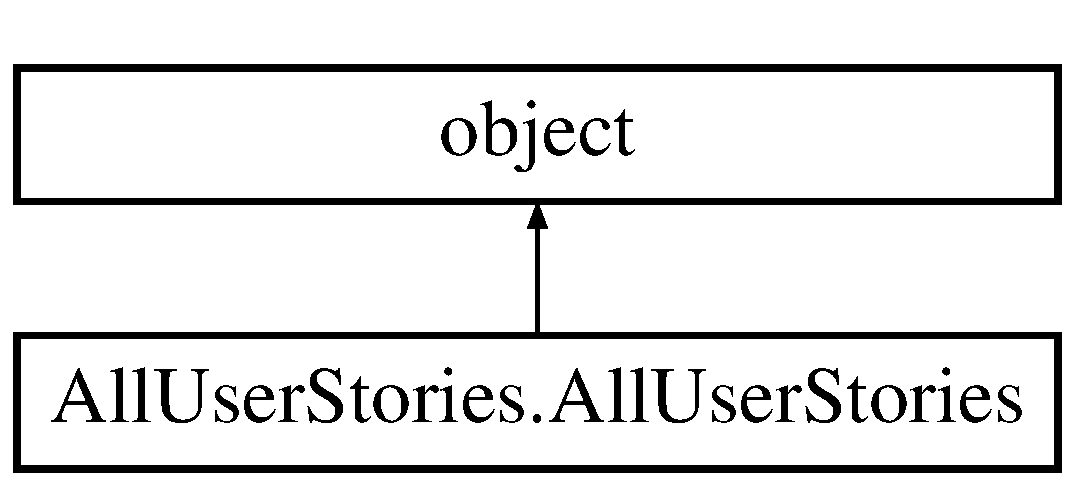
\includegraphics[height=2.000000cm]{class_all_user_stories_1_1_all_user_stories}
\end{center}
\end{figure}
\subsection*{Public Member Functions}
\begin{DoxyCompactItemize}
\item 
\hypertarget{class_all_user_stories_1_1_all_user_stories_a2ae1139002bd6e26a335a57cc2fb6f13}{}\label{class_all_user_stories_1_1_all_user_stories_a2ae1139002bd6e26a335a57cc2fb6f13} 
def {\bfseries \+\_\+\+\_\+init\+\_\+\+\_\+} (self)
\item 
def \hyperlink{class_all_user_stories_1_1_all_user_stories_a70125234edcc5315e8473d9928d85c80}{mongo\+Story1} (self, Mongo\+Queries, G\+UI, cust\+ID)
\item 
def \hyperlink{class_all_user_stories_1_1_all_user_stories_a749505378bf81816d48d6f72553379d1}{mongo\+Story2} (self, Mongo\+Queries, G\+UI, gender)
\item 
def \hyperlink{class_all_user_stories_1_1_all_user_stories_a89b5e3cfc51a5cf4f8299b3c0695824d}{mongo\+Story3} (self, Mongo\+Queries, G\+UI)
\item 
def \hyperlink{class_all_user_stories_1_1_all_user_stories_a1c32ef2b5c7cdac1fe9e6695b77f798f}{mongo\+Story4} (self, Mongo\+Queries, G\+UI, product\+ID)
\item 
def \hyperlink{class_all_user_stories_1_1_all_user_stories_acf328e4938ec594a351ae762464507ad}{mongo\+Story5} (self, Mongo\+Queries, G\+UI)
\item 
def \hyperlink{class_all_user_stories_1_1_all_user_stories_a28910ecdf86a20ec3e21acbc600cfb4f}{mongo\+Story6} (Mongo\+Queries, G\+UI)
\item 
def \hyperlink{class_all_user_stories_1_1_all_user_stories_afce2cf693ebf64cf3e056995968ffe29}{user\+Story12} (self, db, G\+UI, product\+ID)
\item 
def \hyperlink{class_all_user_stories_1_1_all_user_stories_ad0f925eabb44f073abfa723cf10205e7}{user\+Story\+Series1} (self, db, G\+UI, start\+Date, end\+Date, query\+\_\+number)
\item 
def \hyperlink{class_all_user_stories_1_1_all_user_stories_a3652c394b2fcdead6261d92c22109f53}{user\+Story\+Series2} (self, db, G\+UI, start\+Date, end\+Date, additional\+\_\+attribute, query\+\_\+number)
\end{DoxyCompactItemize}


\subsection{Member Function Documentation}
\hypertarget{class_all_user_stories_1_1_all_user_stories_a70125234edcc5315e8473d9928d85c80}{}\label{class_all_user_stories_1_1_all_user_stories_a70125234edcc5315e8473d9928d85c80} 
\index{All\+User\+Stories\+::\+All\+User\+Stories@{All\+User\+Stories\+::\+All\+User\+Stories}!mongo\+Story1@{mongo\+Story1}}
\index{mongo\+Story1@{mongo\+Story1}!All\+User\+Stories\+::\+All\+User\+Stories@{All\+User\+Stories\+::\+All\+User\+Stories}}
\subsubsection{\texorpdfstring{mongo\+Story1()}{mongoStory1()}}
{\footnotesize\ttfamily def All\+User\+Stories.\+All\+User\+Stories.\+mongo\+Story1 (\begin{DoxyParamCaption}\item[{}]{self,  }\item[{}]{Mongo\+Queries,  }\item[{}]{G\+UI,  }\item[{}]{cust\+ID }\end{DoxyParamCaption})}

\begin{DoxyVerb}userStory7(Boolean for GUI, customer id): This method does xyz \end{DoxyVerb}
 \hypertarget{class_all_user_stories_1_1_all_user_stories_a749505378bf81816d48d6f72553379d1}{}\label{class_all_user_stories_1_1_all_user_stories_a749505378bf81816d48d6f72553379d1} 
\index{All\+User\+Stories\+::\+All\+User\+Stories@{All\+User\+Stories\+::\+All\+User\+Stories}!mongo\+Story2@{mongo\+Story2}}
\index{mongo\+Story2@{mongo\+Story2}!All\+User\+Stories\+::\+All\+User\+Stories@{All\+User\+Stories\+::\+All\+User\+Stories}}
\subsubsection{\texorpdfstring{mongo\+Story2()}{mongoStory2()}}
{\footnotesize\ttfamily def All\+User\+Stories.\+All\+User\+Stories.\+mongo\+Story2 (\begin{DoxyParamCaption}\item[{}]{self,  }\item[{}]{Mongo\+Queries,  }\item[{}]{G\+UI,  }\item[{}]{gender }\end{DoxyParamCaption})}

\begin{DoxyVerb}useCase1: Accepts parameter 'period' which is a period, 1-4 \end{DoxyVerb}
 \hypertarget{class_all_user_stories_1_1_all_user_stories_a89b5e3cfc51a5cf4f8299b3c0695824d}{}\label{class_all_user_stories_1_1_all_user_stories_a89b5e3cfc51a5cf4f8299b3c0695824d} 
\index{All\+User\+Stories\+::\+All\+User\+Stories@{All\+User\+Stories\+::\+All\+User\+Stories}!mongo\+Story3@{mongo\+Story3}}
\index{mongo\+Story3@{mongo\+Story3}!All\+User\+Stories\+::\+All\+User\+Stories@{All\+User\+Stories\+::\+All\+User\+Stories}}
\subsubsection{\texorpdfstring{mongo\+Story3()}{mongoStory3()}}
{\footnotesize\ttfamily def All\+User\+Stories.\+All\+User\+Stories.\+mongo\+Story3 (\begin{DoxyParamCaption}\item[{}]{self,  }\item[{}]{Mongo\+Queries,  }\item[{}]{G\+UI }\end{DoxyParamCaption})}

\begin{DoxyVerb}useCase9: \end{DoxyVerb}
 \hypertarget{class_all_user_stories_1_1_all_user_stories_a1c32ef2b5c7cdac1fe9e6695b77f798f}{}\label{class_all_user_stories_1_1_all_user_stories_a1c32ef2b5c7cdac1fe9e6695b77f798f} 
\index{All\+User\+Stories\+::\+All\+User\+Stories@{All\+User\+Stories\+::\+All\+User\+Stories}!mongo\+Story4@{mongo\+Story4}}
\index{mongo\+Story4@{mongo\+Story4}!All\+User\+Stories\+::\+All\+User\+Stories@{All\+User\+Stories\+::\+All\+User\+Stories}}
\subsubsection{\texorpdfstring{mongo\+Story4()}{mongoStory4()}}
{\footnotesize\ttfamily def All\+User\+Stories.\+All\+User\+Stories.\+mongo\+Story4 (\begin{DoxyParamCaption}\item[{}]{self,  }\item[{}]{Mongo\+Queries,  }\item[{}]{G\+UI,  }\item[{}]{product\+ID }\end{DoxyParamCaption})}

\begin{DoxyVerb}useCase10 \end{DoxyVerb}
 \hypertarget{class_all_user_stories_1_1_all_user_stories_acf328e4938ec594a351ae762464507ad}{}\label{class_all_user_stories_1_1_all_user_stories_acf328e4938ec594a351ae762464507ad} 
\index{All\+User\+Stories\+::\+All\+User\+Stories@{All\+User\+Stories\+::\+All\+User\+Stories}!mongo\+Story5@{mongo\+Story5}}
\index{mongo\+Story5@{mongo\+Story5}!All\+User\+Stories\+::\+All\+User\+Stories@{All\+User\+Stories\+::\+All\+User\+Stories}}
\subsubsection{\texorpdfstring{mongo\+Story5()}{mongoStory5()}}
{\footnotesize\ttfamily def All\+User\+Stories.\+All\+User\+Stories.\+mongo\+Story5 (\begin{DoxyParamCaption}\item[{}]{self,  }\item[{}]{Mongo\+Queries,  }\item[{}]{G\+UI }\end{DoxyParamCaption})}

\begin{DoxyVerb}useCase11 \end{DoxyVerb}
 \hypertarget{class_all_user_stories_1_1_all_user_stories_a28910ecdf86a20ec3e21acbc600cfb4f}{}\label{class_all_user_stories_1_1_all_user_stories_a28910ecdf86a20ec3e21acbc600cfb4f} 
\index{All\+User\+Stories\+::\+All\+User\+Stories@{All\+User\+Stories\+::\+All\+User\+Stories}!mongo\+Story6@{mongo\+Story6}}
\index{mongo\+Story6@{mongo\+Story6}!All\+User\+Stories\+::\+All\+User\+Stories@{All\+User\+Stories\+::\+All\+User\+Stories}}
\subsubsection{\texorpdfstring{mongo\+Story6()}{mongoStory6()}}
{\footnotesize\ttfamily def All\+User\+Stories.\+All\+User\+Stories.\+mongo\+Story6 (\begin{DoxyParamCaption}\item[{}]{Mongo\+Queries,  }\item[{}]{G\+UI }\end{DoxyParamCaption})}

\begin{DoxyVerb}useCase15 \end{DoxyVerb}
 \hypertarget{class_all_user_stories_1_1_all_user_stories_afce2cf693ebf64cf3e056995968ffe29}{}\label{class_all_user_stories_1_1_all_user_stories_afce2cf693ebf64cf3e056995968ffe29} 
\index{All\+User\+Stories\+::\+All\+User\+Stories@{All\+User\+Stories\+::\+All\+User\+Stories}!user\+Story12@{user\+Story12}}
\index{user\+Story12@{user\+Story12}!All\+User\+Stories\+::\+All\+User\+Stories@{All\+User\+Stories\+::\+All\+User\+Stories}}
\subsubsection{\texorpdfstring{user\+Story12()}{userStory12()}}
{\footnotesize\ttfamily def All\+User\+Stories.\+All\+User\+Stories.\+user\+Story12 (\begin{DoxyParamCaption}\item[{}]{self,  }\item[{}]{db,  }\item[{}]{G\+UI,  }\item[{}]{product\+ID }\end{DoxyParamCaption})}

\begin{DoxyVerb}useCase1: Accepts parameter 'period' which is a period, 1-4 \end{DoxyVerb}
 \hypertarget{class_all_user_stories_1_1_all_user_stories_ad0f925eabb44f073abfa723cf10205e7}{}\label{class_all_user_stories_1_1_all_user_stories_ad0f925eabb44f073abfa723cf10205e7} 
\index{All\+User\+Stories\+::\+All\+User\+Stories@{All\+User\+Stories\+::\+All\+User\+Stories}!user\+Story\+Series1@{user\+Story\+Series1}}
\index{user\+Story\+Series1@{user\+Story\+Series1}!All\+User\+Stories\+::\+All\+User\+Stories@{All\+User\+Stories\+::\+All\+User\+Stories}}
\subsubsection{\texorpdfstring{user\+Story\+Series1()}{userStorySeries1()}}
{\footnotesize\ttfamily def All\+User\+Stories.\+All\+User\+Stories.\+user\+Story\+Series1 (\begin{DoxyParamCaption}\item[{}]{self,  }\item[{}]{db,  }\item[{}]{G\+UI,  }\item[{}]{start\+Date,  }\item[{}]{end\+Date,  }\item[{}]{query\+\_\+number }\end{DoxyParamCaption})}

\begin{DoxyVerb}useCase1: Accepts parameter 'period' which is a period, 1-4 \end{DoxyVerb}
 \hypertarget{class_all_user_stories_1_1_all_user_stories_a3652c394b2fcdead6261d92c22109f53}{}\label{class_all_user_stories_1_1_all_user_stories_a3652c394b2fcdead6261d92c22109f53} 
\index{All\+User\+Stories\+::\+All\+User\+Stories@{All\+User\+Stories\+::\+All\+User\+Stories}!user\+Story\+Series2@{user\+Story\+Series2}}
\index{user\+Story\+Series2@{user\+Story\+Series2}!All\+User\+Stories\+::\+All\+User\+Stories@{All\+User\+Stories\+::\+All\+User\+Stories}}
\subsubsection{\texorpdfstring{user\+Story\+Series2()}{userStorySeries2()}}
{\footnotesize\ttfamily def All\+User\+Stories.\+All\+User\+Stories.\+user\+Story\+Series2 (\begin{DoxyParamCaption}\item[{}]{self,  }\item[{}]{db,  }\item[{}]{G\+UI,  }\item[{}]{start\+Date,  }\item[{}]{end\+Date,  }\item[{}]{additional\+\_\+attribute,  }\item[{}]{query\+\_\+number }\end{DoxyParamCaption})}

\begin{DoxyVerb}useCase3: Accepts parameter 'period' which is a period, 1-4 \end{DoxyVerb}
 

The documentation for this class was generated from the following file\+:\begin{DoxyCompactItemize}
\item 
src/\+User\+Stories/All\+User\+Stories.\+py\end{DoxyCompactItemize}

\hypertarget{class_mongo_queries_1_1_customer_order_reviews}{}\section{Mongo\+Queries.\+Customer\+Order\+Reviews Class Reference}
\label{class_mongo_queries_1_1_customer_order_reviews}\index{Mongo\+Queries.\+Customer\+Order\+Reviews@{Mongo\+Queries.\+Customer\+Order\+Reviews}}
\subsection*{Public Member Functions}
\begin{DoxyCompactItemize}
\item 
\hypertarget{class_mongo_queries_1_1_customer_order_reviews_a4a6fc6cd2e4ff0421c0c67ac5e57e167}{}\label{class_mongo_queries_1_1_customer_order_reviews_a4a6fc6cd2e4ff0421c0c67ac5e57e167} 
def \hyperlink{class_mongo_queries_1_1_customer_order_reviews_a4a6fc6cd2e4ff0421c0c67ac5e57e167}{get\+Product\+Scores} (i)
\begin{DoxyCompactList}\small\item\em accesses \hyperlink{class_mongo_queries_1_1_product_details}{Product\+Details} Collection \#\#\#\#\# \end{DoxyCompactList}\item 
\hypertarget{class_mongo_queries_1_1_customer_order_reviews_ac347dd548f4ba963a6b8c4edc078ef2f}{}\label{class_mongo_queries_1_1_customer_order_reviews_ac347dd548f4ba963a6b8c4edc078ef2f} 
def {\bfseries get\+Product\+Scoresf\+Cust} (i)
\item 
\hypertarget{class_mongo_queries_1_1_customer_order_reviews_a099e617ee45f23d1927c2eeaaf459745}{}\label{class_mongo_queries_1_1_customer_order_reviews_a099e617ee45f23d1927c2eeaaf459745} 
def {\bfseries get\+Product\+Reviewsf\+Prod} (i)
\item 
\hypertarget{class_mongo_queries_1_1_customer_order_reviews_af30eb76b9151f6a8985822e04d888a76}{}\label{class_mongo_queries_1_1_customer_order_reviews_af30eb76b9151f6a8985822e04d888a76} 
def {\bfseries get\+Product\+Reviewsf\+Cust} (i)
\item 
\hypertarget{class_mongo_queries_1_1_customer_order_reviews_ab679e16849111b5fe3ecccc9aeadab02}{}\label{class_mongo_queries_1_1_customer_order_reviews_ab679e16849111b5fe3ecccc9aeadab02} 
def {\bfseries get\+Service\+Score} (i)
\item 
\hypertarget{class_mongo_queries_1_1_customer_order_reviews_ac6c9d968c69ffa58c6594f56a35024d7}{}\label{class_mongo_queries_1_1_customer_order_reviews_ac6c9d968c69ffa58c6594f56a35024d7} 
def {\bfseries get\+Delivery\+Score} (i)
\end{DoxyCompactItemize}


The documentation for this class was generated from the following file\+:\begin{DoxyCompactItemize}
\item 
src/mongo\+Database/Mongo\+Queries.\+py\end{DoxyCompactItemize}

\hypertarget{class_login_1_1_login}{}\section{Login.\+Login Class Reference}
\label{class_login_1_1_login}\index{Login.\+Login@{Login.\+Login}}
Inheritance diagram for Login.\+Login\+:\begin{figure}[H]
\begin{center}
\leavevmode
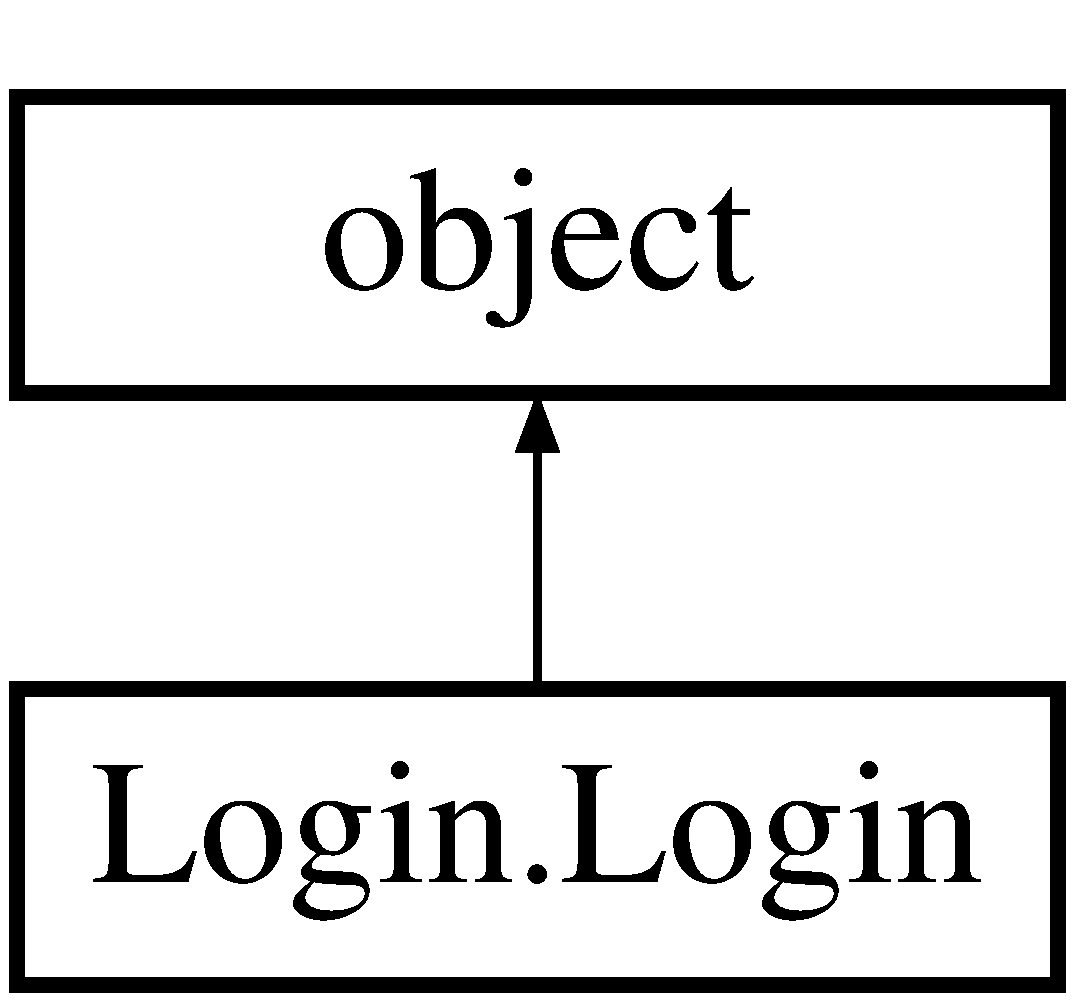
\includegraphics[height=2.000000cm]{class_login_1_1_login}
\end{center}
\end{figure}
\subsection*{Public Member Functions}
\begin{DoxyCompactItemize}
\item 
\hypertarget{class_login_1_1_login_a74dca9aa3c7fc04833737bed7ba4f48d}{}\label{class_login_1_1_login_a74dca9aa3c7fc04833737bed7ba4f48d} 
def {\bfseries \+\_\+\+\_\+init\+\_\+\+\_\+} (self)
\item 
def \hyperlink{class_login_1_1_login_a77f5c43218a5b49e663f72e02324b8ef}{print\+Welcome} (self)
\item 
def \hyperlink{class_login_1_1_login_a21cb771ec1b1d2d7aa17ca541465200b}{get\+Username} (self)
\item 
def \hyperlink{class_login_1_1_login_a61681c3cd7aae627d5a41324ba0f9d76}{get\+Password} (self)
\item 
def \hyperlink{class_login_1_1_login_a4ccae6933e82c3ff7d7cb257427064e2}{get\+Login\+Details} (self)
\end{DoxyCompactItemize}
\subsection*{Public Attributes}
\begin{DoxyCompactItemize}
\item 
\hypertarget{class_login_1_1_login_a17601e10f372715b555b073bcb7cf407}{}\label{class_login_1_1_login_a17601e10f372715b555b073bcb7cf407} 
{\bfseries username}
\item 
\hypertarget{class_login_1_1_login_a02c4b71b842db75f807a06fd79549bcc}{}\label{class_login_1_1_login_a02c4b71b842db75f807a06fd79549bcc} 
{\bfseries password}
\end{DoxyCompactItemize}


\subsection{Detailed Description}
\begin{DoxyVerb}Login: Gets user login details and returns them in a string \end{DoxyVerb}
 

\subsection{Member Function Documentation}
\hypertarget{class_login_1_1_login_a4ccae6933e82c3ff7d7cb257427064e2}{}\label{class_login_1_1_login_a4ccae6933e82c3ff7d7cb257427064e2} 
\index{Login\+::\+Login@{Login\+::\+Login}!get\+Login\+Details@{get\+Login\+Details}}
\index{get\+Login\+Details@{get\+Login\+Details}!Login\+::\+Login@{Login\+::\+Login}}
\subsubsection{\texorpdfstring{get\+Login\+Details()}{getLoginDetails()}}
{\footnotesize\ttfamily def Login.\+Login.\+get\+Login\+Details (\begin{DoxyParamCaption}\item[{}]{self }\end{DoxyParamCaption})}

\begin{DoxyVerb}getLoginDetails: Simply returns a list with user/password  \end{DoxyVerb}
 \hypertarget{class_login_1_1_login_a61681c3cd7aae627d5a41324ba0f9d76}{}\label{class_login_1_1_login_a61681c3cd7aae627d5a41324ba0f9d76} 
\index{Login\+::\+Login@{Login\+::\+Login}!get\+Password@{get\+Password}}
\index{get\+Password@{get\+Password}!Login\+::\+Login@{Login\+::\+Login}}
\subsubsection{\texorpdfstring{get\+Password()}{getPassword()}}
{\footnotesize\ttfamily def Login.\+Login.\+get\+Password (\begin{DoxyParamCaption}\item[{}]{self }\end{DoxyParamCaption})}

\begin{DoxyVerb}getPassword: Get userinput for the password, getpass module 
    should be used to print '*'s as the user types in password,
    this doesn't work in Spyder IDE though. \end{DoxyVerb}
 \hypertarget{class_login_1_1_login_a21cb771ec1b1d2d7aa17ca541465200b}{}\label{class_login_1_1_login_a21cb771ec1b1d2d7aa17ca541465200b} 
\index{Login\+::\+Login@{Login\+::\+Login}!get\+Username@{get\+Username}}
\index{get\+Username@{get\+Username}!Login\+::\+Login@{Login\+::\+Login}}
\subsubsection{\texorpdfstring{get\+Username()}{getUsername()}}
{\footnotesize\ttfamily def Login.\+Login.\+get\+Username (\begin{DoxyParamCaption}\item[{}]{self }\end{DoxyParamCaption})}

\begin{DoxyVerb}getUsername: Get userinput for the username \end{DoxyVerb}
 \hypertarget{class_login_1_1_login_a77f5c43218a5b49e663f72e02324b8ef}{}\label{class_login_1_1_login_a77f5c43218a5b49e663f72e02324b8ef} 
\index{Login\+::\+Login@{Login\+::\+Login}!print\+Welcome@{print\+Welcome}}
\index{print\+Welcome@{print\+Welcome}!Login\+::\+Login@{Login\+::\+Login}}
\subsubsection{\texorpdfstring{print\+Welcome()}{printWelcome()}}
{\footnotesize\ttfamily def Login.\+Login.\+print\+Welcome (\begin{DoxyParamCaption}\item[{}]{self }\end{DoxyParamCaption})}

\begin{DoxyVerb}printWelcome: Prints the welcome message \end{DoxyVerb}
 

The documentation for this class was generated from the following file\+:\begin{DoxyCompactItemize}
\item 
src/Login.\+py\end{DoxyCompactItemize}

\hypertarget{classmain_g_u_i_1_1_main_application}{}\section{main\+G\+U\+I.\+Main\+Application Class Reference}
\label{classmain_g_u_i_1_1_main_application}\index{main\+G\+U\+I.\+Main\+Application@{main\+G\+U\+I.\+Main\+Application}}
Inheritance diagram for main\+G\+U\+I.\+Main\+Application\+:\begin{figure}[H]
\begin{center}
\leavevmode
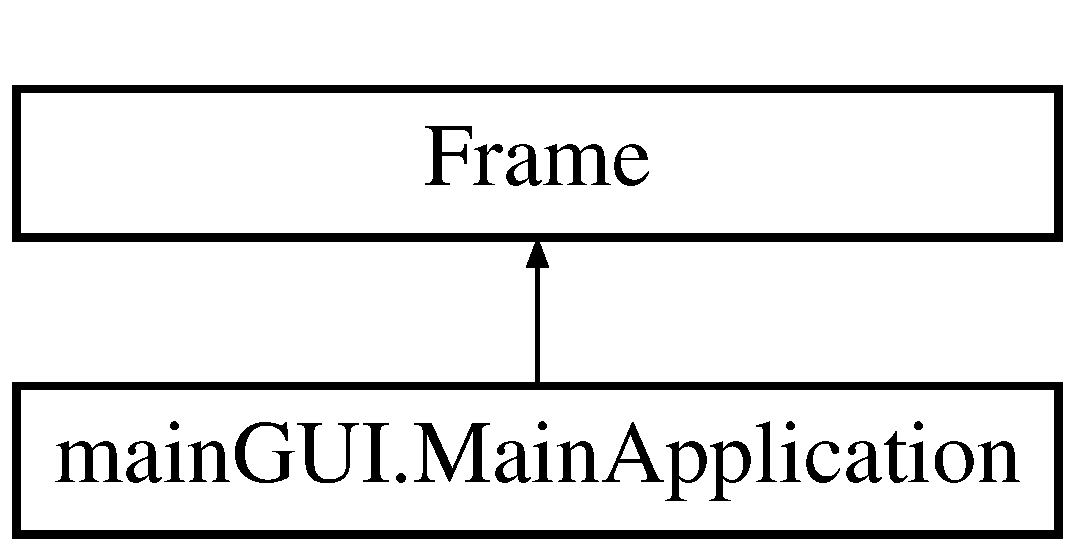
\includegraphics[height=2.000000cm]{classmain_g_u_i_1_1_main_application}
\end{center}
\end{figure}
\subsection*{Public Member Functions}
\begin{DoxyCompactItemize}
\item 
\hypertarget{classmain_g_u_i_1_1_main_application_acac3bbf3ac2feae88abdf108ec7d41e0}{}\label{classmain_g_u_i_1_1_main_application_acac3bbf3ac2feae88abdf108ec7d41e0} 
def {\bfseries \+\_\+\+\_\+init\+\_\+\+\_\+} (self, master, args, kwargs)
\item 
def \hyperlink{classmain_g_u_i_1_1_main_application_a828c13a008e6029d6f9aac3d3f6189fd}{submit} (self)
\item 
def \hyperlink{classmain_g_u_i_1_1_main_application_a8389dd29b6914c6e878435ba3176f2af}{on\+Entry\+Click} (self, event, tk\+Widget\+Name)
\item 
\hypertarget{classmain_g_u_i_1_1_main_application_a338c7e4b5eb933d02649355337da1250}{}\label{classmain_g_u_i_1_1_main_application_a338c7e4b5eb933d02649355337da1250} 
def {\bfseries set\+Current\+Drop\+Down\+Menu\+No} (self, no)
\item 
\hypertarget{classmain_g_u_i_1_1_main_application_a32456a8dcc69bf8b72d3c42e8ec9b8f1}{}\label{classmain_g_u_i_1_1_main_application_a32456a8dcc69bf8b72d3c42e8ec9b8f1} 
def {\bfseries submit\+User\+Story} (self, user\+Story\+No)
\item 
def \hyperlink{classmain_g_u_i_1_1_main_application_af3fa9d6210d07607eb8161acd340eed0}{logout} (self)
\item 
def \hyperlink{classmain_g_u_i_1_1_main_application_a47ac9da75d8ab9ecd89b3e7590ccf754}{custom\+S\+QL} (self)
\item 
def \hyperlink{classmain_g_u_i_1_1_main_application_adfb6937d77ab2cde3eb371057482ab6e}{custom\+Mongo} (self)
\end{DoxyCompactItemize}
\subsection*{Public Attributes}
\begin{DoxyCompactItemize}
\item 
\hypertarget{classmain_g_u_i_1_1_main_application_a1ad4fa8a789e2c8b37cebde17195bcb4}{}\label{classmain_g_u_i_1_1_main_application_a1ad4fa8a789e2c8b37cebde17195bcb4} 
{\bfseries master}
\item 
\hypertarget{classmain_g_u_i_1_1_main_application_af1b6e167eb4cd674ef67a84c279a602a}{}\label{classmain_g_u_i_1_1_main_application_af1b6e167eb4cd674ef67a84c279a602a} 
{\bfseries first\+Click}
\item 
\hypertarget{classmain_g_u_i_1_1_main_application_a3adb73c49afec216252d611359d949f0}{}\label{classmain_g_u_i_1_1_main_application_a3adb73c49afec216252d611359d949f0} 
{\bfseries menu\+Lines}
\item 
\hypertarget{classmain_g_u_i_1_1_main_application_a49fa6014909e7a01877823ce4fa86014}{}\label{classmain_g_u_i_1_1_main_application_a49fa6014909e7a01877823ce4fa86014} 
{\bfseries nb\+Title}
\item 
\hypertarget{classmain_g_u_i_1_1_main_application_a82e73299ec3ece45d5656e275002efe5}{}\label{classmain_g_u_i_1_1_main_application_a82e73299ec3ece45d5656e275002efe5} 
{\bfseries main\+Text}
\item 
\hypertarget{classmain_g_u_i_1_1_main_application_a925c2025c7a39765deed67583a6dc3cf}{}\label{classmain_g_u_i_1_1_main_application_a925c2025c7a39765deed67583a6dc3cf} 
{\bfseries sql\+Label}
\item 
\hypertarget{classmain_g_u_i_1_1_main_application_ac5d1d72fc8c147f637053fcfee51308e}{}\label{classmain_g_u_i_1_1_main_application_ac5d1d72fc8c147f637053fcfee51308e} 
{\bfseries username\+Label}
\item 
\hypertarget{classmain_g_u_i_1_1_main_application_a07e55583875a32c1300eee88cd58168b}{}\label{classmain_g_u_i_1_1_main_application_a07e55583875a32c1300eee88cd58168b} 
{\bfseries username\+Entry}
\item 
\hypertarget{classmain_g_u_i_1_1_main_application_a7b3e6a19bc2151af61904a2c2fb145af}{}\label{classmain_g_u_i_1_1_main_application_a7b3e6a19bc2151af61904a2c2fb145af} 
{\bfseries password\+Label}
\item 
\hypertarget{classmain_g_u_i_1_1_main_application_acf79b09605cc45b4f697fbb2c9d51f02}{}\label{classmain_g_u_i_1_1_main_application_acf79b09605cc45b4f697fbb2c9d51f02} 
{\bfseries password\+Entry}
\item 
\hypertarget{classmain_g_u_i_1_1_main_application_aac99e80a4c81758208c0582fee178c48}{}\label{classmain_g_u_i_1_1_main_application_aac99e80a4c81758208c0582fee178c48} 
{\bfseries submit\+Button}
\item 
\hypertarget{classmain_g_u_i_1_1_main_application_a4b26910056eafff70514625d505c0435}{}\label{classmain_g_u_i_1_1_main_application_a4b26910056eafff70514625d505c0435} 
{\bfseries logout\+Button}
\item 
\hypertarget{classmain_g_u_i_1_1_main_application_ae4c732e3c7a2d46f3be57b273658fadd}{}\label{classmain_g_u_i_1_1_main_application_ae4c732e3c7a2d46f3be57b273658fadd} 
{\bfseries login\+Status\+Label}
\item 
\hypertarget{classmain_g_u_i_1_1_main_application_a154af26bbf690da3b3e8016a9270ab7d}{}\label{classmain_g_u_i_1_1_main_application_a154af26bbf690da3b3e8016a9270ab7d} 
{\bfseries db}
\item 
\hypertarget{classmain_g_u_i_1_1_main_application_ab8265ff450f083500e328b54ac55f643}{}\label{classmain_g_u_i_1_1_main_application_ab8265ff450f083500e328b54ac55f643} 
{\bfseries mongo\+DB}
\item 
\hypertarget{classmain_g_u_i_1_1_main_application_adc26da0ac2aeea9428144733655dbd06}{}\label{classmain_g_u_i_1_1_main_application_adc26da0ac2aeea9428144733655dbd06} 
{\bfseries custom\+Query\+Label}
\item 
\hypertarget{classmain_g_u_i_1_1_main_application_aab030eb7275e25c8af88733e23353991}{}\label{classmain_g_u_i_1_1_main_application_aab030eb7275e25c8af88733e23353991} 
{\bfseries custom\+Query\+Entry}
\item 
\hypertarget{classmain_g_u_i_1_1_main_application_a14c0a7cd4eff699785dfcfe1a0044fff}{}\label{classmain_g_u_i_1_1_main_application_a14c0a7cd4eff699785dfcfe1a0044fff} 
{\bfseries custom\+Query\+Button}
\item 
\hypertarget{classmain_g_u_i_1_1_main_application_ab7091bdbf34163fc8065b54148e4c3d1}{}\label{classmain_g_u_i_1_1_main_application_ab7091bdbf34163fc8065b54148e4c3d1} 
{\bfseries custom\+Query\+Button\+Mongo}
\item 
\hypertarget{classmain_g_u_i_1_1_main_application_aa3a89fa2f075e7d03f8d818d400fe378}{}\label{classmain_g_u_i_1_1_main_application_aa3a89fa2f075e7d03f8d818d400fe378} 
{\bfseries spacer\+Label0}
\item 
\hypertarget{classmain_g_u_i_1_1_main_application_a549a4a9fc1738b707a605cda4924f9e5}{}\label{classmain_g_u_i_1_1_main_application_a549a4a9fc1738b707a605cda4924f9e5} 
{\bfseries drop}
\item 
\hypertarget{classmain_g_u_i_1_1_main_application_a9e0d95c2146f4c3c648ebc613854b0ba}{}\label{classmain_g_u_i_1_1_main_application_a9e0d95c2146f4c3c648ebc613854b0ba} 
{\bfseries spacer\+Label1}
\item 
\hypertarget{classmain_g_u_i_1_1_main_application_af20185ebf2a33d11519f10aa53abce17}{}\label{classmain_g_u_i_1_1_main_application_af20185ebf2a33d11519f10aa53abce17} 
{\bfseries query\+Input\+Box1}
\item 
\hypertarget{classmain_g_u_i_1_1_main_application_ac74a832fe09a62ce7b1115cc88928f12}{}\label{classmain_g_u_i_1_1_main_application_ac74a832fe09a62ce7b1115cc88928f12} 
{\bfseries query\+Input\+Box2}
\item 
\hypertarget{classmain_g_u_i_1_1_main_application_a07bc20d647585d2a0c23943aef42b570}{}\label{classmain_g_u_i_1_1_main_application_a07bc20d647585d2a0c23943aef42b570} 
{\bfseries query\+Input\+Box3}
\item 
\hypertarget{classmain_g_u_i_1_1_main_application_a6cc2b89071419d90c1b98fa8d95df2df}{}\label{classmain_g_u_i_1_1_main_application_a6cc2b89071419d90c1b98fa8d95df2df} 
{\bfseries submit\+User\+Story\+Inputs}
\item 
\hypertarget{classmain_g_u_i_1_1_main_application_a86dfd0f97f8952cdde81bf89efab6e68}{}\label{classmain_g_u_i_1_1_main_application_a86dfd0f97f8952cdde81bf89efab6e68} 
{\bfseries query\+Result\+Box}
\end{DoxyCompactItemize}


\subsection{Detailed Description}
\begin{DoxyVerb}MainApplication: Provides the main logic for the GUI, allows the
    user to log in with user/password, before executing SQL queries. \end{DoxyVerb}
 

\subsection{Member Function Documentation}
\hypertarget{classmain_g_u_i_1_1_main_application_adfb6937d77ab2cde3eb371057482ab6e}{}\label{classmain_g_u_i_1_1_main_application_adfb6937d77ab2cde3eb371057482ab6e} 
\index{main\+G\+U\+I\+::\+Main\+Application@{main\+G\+U\+I\+::\+Main\+Application}!custom\+Mongo@{custom\+Mongo}}
\index{custom\+Mongo@{custom\+Mongo}!main\+G\+U\+I\+::\+Main\+Application@{main\+G\+U\+I\+::\+Main\+Application}}
\subsubsection{\texorpdfstring{custom\+Mongo()}{customMongo()}}
{\footnotesize\ttfamily def main\+G\+U\+I.\+Main\+Application.\+custom\+Mongo (\begin{DoxyParamCaption}\item[{}]{self }\end{DoxyParamCaption})}

\begin{DoxyVerb}customSQL: Allows custom SQL queries to be input, sends user input
    to method in MySQLDatabase, results returned in toPrint. Results
    printed on new lines using eval(). \end{DoxyVerb}
 \hypertarget{classmain_g_u_i_1_1_main_application_a47ac9da75d8ab9ecd89b3e7590ccf754}{}\label{classmain_g_u_i_1_1_main_application_a47ac9da75d8ab9ecd89b3e7590ccf754} 
\index{main\+G\+U\+I\+::\+Main\+Application@{main\+G\+U\+I\+::\+Main\+Application}!custom\+S\+QL@{custom\+S\+QL}}
\index{custom\+S\+QL@{custom\+S\+QL}!main\+G\+U\+I\+::\+Main\+Application@{main\+G\+U\+I\+::\+Main\+Application}}
\subsubsection{\texorpdfstring{custom\+S\+Q\+L()}{customSQL()}}
{\footnotesize\ttfamily def main\+G\+U\+I.\+Main\+Application.\+custom\+S\+QL (\begin{DoxyParamCaption}\item[{}]{self }\end{DoxyParamCaption})}

\begin{DoxyVerb}customSQL: Allows custom SQL queries to be input, sends user input
    to method in MySQLDatabase, results returned in toPrint. Results
    printed on new lines using eval(). \end{DoxyVerb}
 \hypertarget{classmain_g_u_i_1_1_main_application_af3fa9d6210d07607eb8161acd340eed0}{}\label{classmain_g_u_i_1_1_main_application_af3fa9d6210d07607eb8161acd340eed0} 
\index{main\+G\+U\+I\+::\+Main\+Application@{main\+G\+U\+I\+::\+Main\+Application}!logout@{logout}}
\index{logout@{logout}!main\+G\+U\+I\+::\+Main\+Application@{main\+G\+U\+I\+::\+Main\+Application}}
\subsubsection{\texorpdfstring{logout()}{logout()}}
{\footnotesize\ttfamily def main\+G\+U\+I.\+Main\+Application.\+logout (\begin{DoxyParamCaption}\item[{}]{self }\end{DoxyParamCaption})}

\begin{DoxyVerb}logout: Destroys GUI features on logout, changes loginStatus label
    text and enable login button and user/password inputs. \end{DoxyVerb}
 \hypertarget{classmain_g_u_i_1_1_main_application_a8389dd29b6914c6e878435ba3176f2af}{}\label{classmain_g_u_i_1_1_main_application_a8389dd29b6914c6e878435ba3176f2af} 
\index{main\+G\+U\+I\+::\+Main\+Application@{main\+G\+U\+I\+::\+Main\+Application}!on\+Entry\+Click@{on\+Entry\+Click}}
\index{on\+Entry\+Click@{on\+Entry\+Click}!main\+G\+U\+I\+::\+Main\+Application@{main\+G\+U\+I\+::\+Main\+Application}}
\subsubsection{\texorpdfstring{on\+Entry\+Click()}{onEntryClick()}}
{\footnotesize\ttfamily def main\+G\+U\+I.\+Main\+Application.\+on\+Entry\+Click (\begin{DoxyParamCaption}\item[{}]{self,  }\item[{}]{event,  }\item[{}]{tk\+Widget\+Name }\end{DoxyParamCaption})}

\begin{DoxyVerb}onEntryClick: onFocus event will delete prompt text in entry box \end{DoxyVerb}
 \hypertarget{classmain_g_u_i_1_1_main_application_a828c13a008e6029d6f9aac3d3f6189fd}{}\label{classmain_g_u_i_1_1_main_application_a828c13a008e6029d6f9aac3d3f6189fd} 
\index{main\+G\+U\+I\+::\+Main\+Application@{main\+G\+U\+I\+::\+Main\+Application}!submit@{submit}}
\index{submit@{submit}!main\+G\+U\+I\+::\+Main\+Application@{main\+G\+U\+I\+::\+Main\+Application}}
\subsubsection{\texorpdfstring{submit()}{submit()}}
{\footnotesize\ttfamily def main\+G\+U\+I.\+Main\+Application.\+submit (\begin{DoxyParamCaption}\item[{}]{self }\end{DoxyParamCaption})}

\begin{DoxyVerb}submit: Submits the user/password to MySQL database, will update
    the loginStatus text on login or failed login. Once the user is
    logged in, the login buttons are disabled. \end{DoxyVerb}
 

The documentation for this class was generated from the following file\+:\begin{DoxyCompactItemize}
\item 
src/main\+G\+U\+I.\+py\end{DoxyCompactItemize}

\hypertarget{classmain_t_u_i_1_1_main_logic}{}\section{main\+T\+U\+I.\+Main\+Logic Class Reference}
\label{classmain_t_u_i_1_1_main_logic}\index{main\+T\+U\+I.\+Main\+Logic@{main\+T\+U\+I.\+Main\+Logic}}
Inheritance diagram for main\+T\+U\+I.\+Main\+Logic\+:\begin{figure}[H]
\begin{center}
\leavevmode
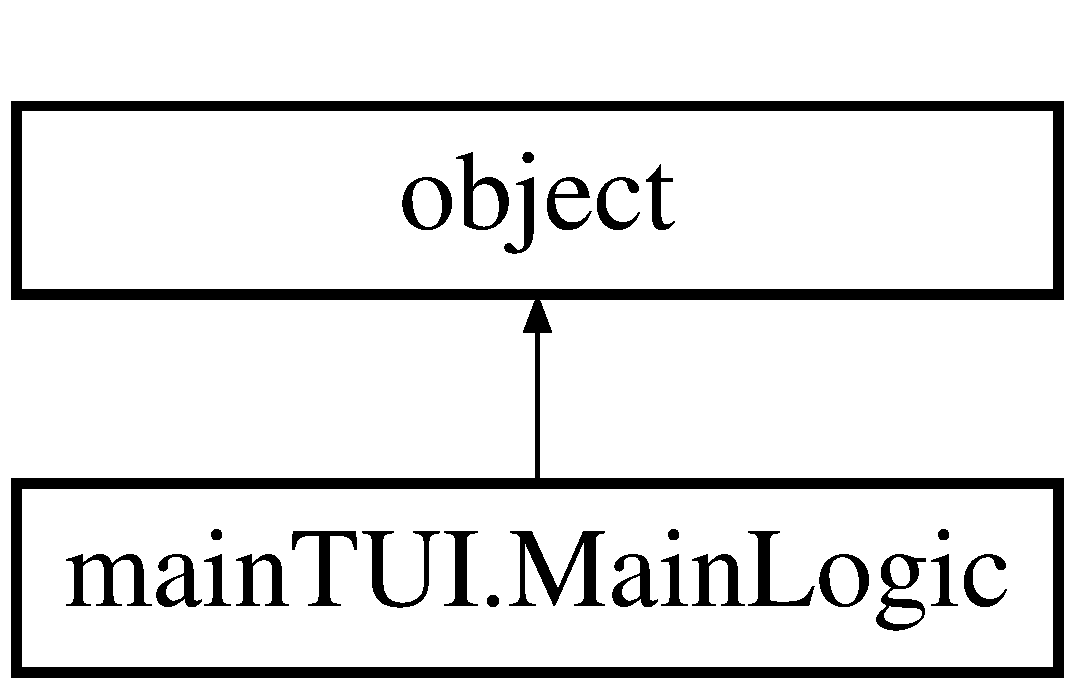
\includegraphics[height=2.000000cm]{classmain_t_u_i_1_1_main_logic}
\end{center}
\end{figure}
\subsection*{Public Member Functions}
\begin{DoxyCompactItemize}
\item 
\hypertarget{classmain_t_u_i_1_1_main_logic_a56aeaabebe5a505379f188d266258979}{}\label{classmain_t_u_i_1_1_main_logic_a56aeaabebe5a505379f188d266258979} 
def {\bfseries \+\_\+\+\_\+init\+\_\+\+\_\+} (self)
\item 
def \hyperlink{classmain_t_u_i_1_1_main_logic_a174991d65104326c736a0d8e3c3e8edd}{run\+Program} (self)
\item 
def \hyperlink{classmain_t_u_i_1_1_main_logic_a0850095d67fa526a848768588eb06ea6}{print\+Menu} (self)
\item 
def \hyperlink{classmain_t_u_i_1_1_main_logic_a91c2a1b004ea6a497dd81ed41528c650}{print\+Gnome} (self)
\item 
def \hyperlink{classmain_t_u_i_1_1_main_logic_ab5d87725a59118bc0816a8a1dd21f06f}{get\+Menu\+Input} (self)
\end{DoxyCompactItemize}
\subsection*{Public Attributes}
\begin{DoxyCompactItemize}
\item 
\hypertarget{classmain_t_u_i_1_1_main_logic_af22c744bd91e1f06fe254936f45ea4b2}{}\label{classmain_t_u_i_1_1_main_logic_af22c744bd91e1f06fe254936f45ea4b2} 
{\bfseries menu\+Lines}
\item 
\hypertarget{classmain_t_u_i_1_1_main_logic_a4cbf963e6d6b4e98fd8eec7c131f3976}{}\label{classmain_t_u_i_1_1_main_logic_a4cbf963e6d6b4e98fd8eec7c131f3976} 
{\bfseries menu\+Option}
\end{DoxyCompactItemize}


\subsection{Detailed Description}
\begin{DoxyVerb}MainLogic: Holds the logic for running the program in the prompt.  \end{DoxyVerb}
 

\subsection{Member Function Documentation}
\hypertarget{classmain_t_u_i_1_1_main_logic_ab5d87725a59118bc0816a8a1dd21f06f}{}\label{classmain_t_u_i_1_1_main_logic_ab5d87725a59118bc0816a8a1dd21f06f} 
\index{main\+T\+U\+I\+::\+Main\+Logic@{main\+T\+U\+I\+::\+Main\+Logic}!get\+Menu\+Input@{get\+Menu\+Input}}
\index{get\+Menu\+Input@{get\+Menu\+Input}!main\+T\+U\+I\+::\+Main\+Logic@{main\+T\+U\+I\+::\+Main\+Logic}}
\subsubsection{\texorpdfstring{get\+Menu\+Input()}{getMenuInput()}}
{\footnotesize\ttfamily def main\+T\+U\+I.\+Main\+Logic.\+get\+Menu\+Input (\begin{DoxyParamCaption}\item[{}]{self }\end{DoxyParamCaption})}

\begin{DoxyVerb}getMenuInput: Gets user input for the menu, returns True/False. \end{DoxyVerb}
 \hypertarget{classmain_t_u_i_1_1_main_logic_a91c2a1b004ea6a497dd81ed41528c650}{}\label{classmain_t_u_i_1_1_main_logic_a91c2a1b004ea6a497dd81ed41528c650} 
\index{main\+T\+U\+I\+::\+Main\+Logic@{main\+T\+U\+I\+::\+Main\+Logic}!print\+Gnome@{print\+Gnome}}
\index{print\+Gnome@{print\+Gnome}!main\+T\+U\+I\+::\+Main\+Logic@{main\+T\+U\+I\+::\+Main\+Logic}}
\subsubsection{\texorpdfstring{print\+Gnome()}{printGnome()}}
{\footnotesize\ttfamily def main\+T\+U\+I.\+Main\+Logic.\+print\+Gnome (\begin{DoxyParamCaption}\item[{}]{self }\end{DoxyParamCaption})}

\begin{DoxyVerb}printGnome: Reads text file containing gnome in ASCII text and
    prints it out, stripping out newline characters. \end{DoxyVerb}
 \hypertarget{classmain_t_u_i_1_1_main_logic_a0850095d67fa526a848768588eb06ea6}{}\label{classmain_t_u_i_1_1_main_logic_a0850095d67fa526a848768588eb06ea6} 
\index{main\+T\+U\+I\+::\+Main\+Logic@{main\+T\+U\+I\+::\+Main\+Logic}!print\+Menu@{print\+Menu}}
\index{print\+Menu@{print\+Menu}!main\+T\+U\+I\+::\+Main\+Logic@{main\+T\+U\+I\+::\+Main\+Logic}}
\subsubsection{\texorpdfstring{print\+Menu()}{printMenu()}}
{\footnotesize\ttfamily def main\+T\+U\+I.\+Main\+Logic.\+print\+Menu (\begin{DoxyParamCaption}\item[{}]{self }\end{DoxyParamCaption})}

\begin{DoxyVerb}printMenu: Prints the main menu. \end{DoxyVerb}
 \hypertarget{classmain_t_u_i_1_1_main_logic_a174991d65104326c736a0d8e3c3e8edd}{}\label{classmain_t_u_i_1_1_main_logic_a174991d65104326c736a0d8e3c3e8edd} 
\index{main\+T\+U\+I\+::\+Main\+Logic@{main\+T\+U\+I\+::\+Main\+Logic}!run\+Program@{run\+Program}}
\index{run\+Program@{run\+Program}!main\+T\+U\+I\+::\+Main\+Logic@{main\+T\+U\+I\+::\+Main\+Logic}}
\subsubsection{\texorpdfstring{run\+Program()}{runProgram()}}
{\footnotesize\ttfamily def main\+T\+U\+I.\+Main\+Logic.\+run\+Program (\begin{DoxyParamCaption}\item[{}]{self }\end{DoxyParamCaption})}

\begin{DoxyVerb}runProgram: Holds logic for the menu choices. \end{DoxyVerb}
 

The documentation for this class was generated from the following file\+:\begin{DoxyCompactItemize}
\item 
src/main\+T\+U\+I.\+py\end{DoxyCompactItemize}

\hypertarget{class_mongo_database_1_1_mongo_database}{}\section{Mongo\+Database.\+Mongo\+Database Class Reference}
\label{class_mongo_database_1_1_mongo_database}\index{Mongo\+Database.\+Mongo\+Database@{Mongo\+Database.\+Mongo\+Database}}
Inheritance diagram for Mongo\+Database.\+Mongo\+Database\+:\begin{figure}[H]
\begin{center}
\leavevmode
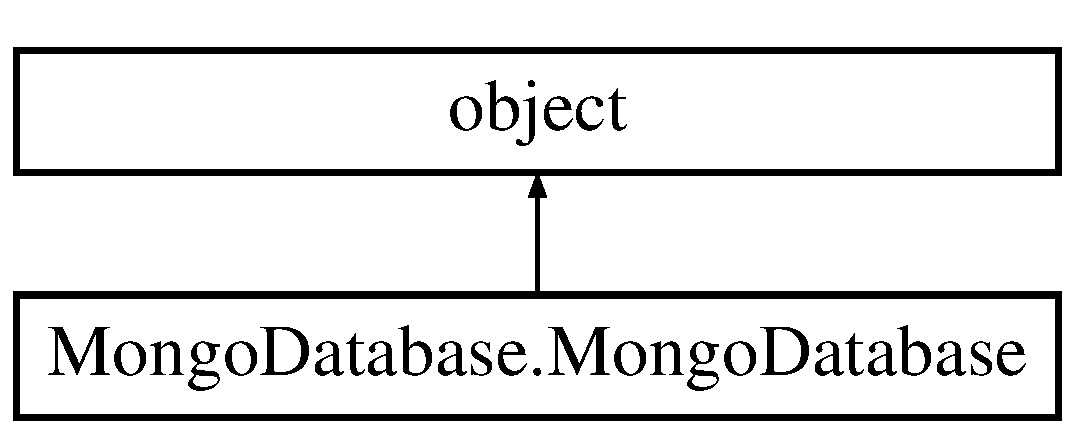
\includegraphics[height=2.000000cm]{class_mongo_database_1_1_mongo_database}
\end{center}
\end{figure}
\subsection*{Public Member Functions}
\begin{DoxyCompactItemize}
\item 
\hypertarget{class_mongo_database_1_1_mongo_database_a02dc685b883d5747c2a8329d4d4c67b5}{}\label{class_mongo_database_1_1_mongo_database_a02dc685b883d5747c2a8329d4d4c67b5} 
def {\bfseries \+\_\+\+\_\+init\+\_\+\+\_\+} (self)
\item 
\hypertarget{class_mongo_database_1_1_mongo_database_a6a22d9c25edbbd88115bbc64889f854d}{}\label{class_mongo_database_1_1_mongo_database_a6a22d9c25edbbd88115bbc64889f854d} 
def {\bfseries method\+Finder} (self)
\item 
def \hyperlink{class_mongo_database_1_1_mongo_database_afdd3078ad8bb851bab945b1b477f1529}{run} (self)
\item 
def \hyperlink{class_mongo_database_1_1_mongo_database_a54df0dccd3550bc038fa246ee0f97a15}{login} (self)
\item 
def \hyperlink{class_mongo_database_1_1_mongo_database_a2eb4c5b675b39a871dfdf03458376363}{print\+Menu} (self)
\item 
def \hyperlink{class_mongo_database_1_1_mongo_database_ab5d6d51b956790d3804e4c566ae40cfe}{get\+Menu\+Input} (self)
\item 
def \hyperlink{class_mongo_database_1_1_mongo_database_a123d046fd01db4d2b342289a972e8e31}{main\+Logic} (self)
\item 
\hypertarget{class_mongo_database_1_1_mongo_database_a80a8491e446682c7e420fd1270c8cfe2}{}\label{class_mongo_database_1_1_mongo_database_a80a8491e446682c7e420fd1270c8cfe2} 
def {\bfseries exit\+Program} (self)
\item 
def \hyperlink{class_mongo_database_1_1_mongo_database_af1be85a82838d6e46f181af707892606}{custom\+Query} (self, G\+UI, user\+Input)
\item 
def \hyperlink{class_mongo_database_1_1_mongo_database_a27e20258620a2a1953a460e7c7aa3e14}{to\+C\+SV} (self, dates, ratings)
\end{DoxyCompactItemize}
\subsection*{Public Attributes}
\begin{DoxyCompactItemize}
\item 
\hypertarget{class_mongo_database_1_1_mongo_database_ac6b838c7e0c2357101e8e8db0dc94aa4}{}\label{class_mongo_database_1_1_mongo_database_ac6b838c7e0c2357101e8e8db0dc94aa4} 
{\bfseries conn}
\item 
\hypertarget{class_mongo_database_1_1_mongo_database_a6de8929dee773729992475177f062af8}{}\label{class_mongo_database_1_1_mongo_database_a6de8929dee773729992475177f062af8} 
{\bfseries menu\+Lines}
\item 
\hypertarget{class_mongo_database_1_1_mongo_database_ab4aeb0410a6d8f6fcdebb4f40ec68c48}{}\label{class_mongo_database_1_1_mongo_database_ab4aeb0410a6d8f6fcdebb4f40ec68c48} 
{\bfseries back\+To\+Main}
\item 
\hypertarget{class_mongo_database_1_1_mongo_database_ad8b5437c836f2ea68938f98431ae2028}{}\label{class_mongo_database_1_1_mongo_database_ad8b5437c836f2ea68938f98431ae2028} 
{\bfseries run\+\_\+mongo\+\_\+query}
\item 
\hypertarget{class_mongo_database_1_1_mongo_database_a2fb2dbb70d9b350dc0183c4f5da9f396}{}\label{class_mongo_database_1_1_mongo_database_a2fb2dbb70d9b350dc0183c4f5da9f396} 
{\bfseries menu\+Option}
\end{DoxyCompactItemize}


\subsection{Detailed Description}
\begin{DoxyVerb}Database: Holds the database object used for querying. Prints the menu
    for the Mongo options, executes custom query. \end{DoxyVerb}
 

\subsection{Member Function Documentation}
\hypertarget{class_mongo_database_1_1_mongo_database_af1be85a82838d6e46f181af707892606}{}\label{class_mongo_database_1_1_mongo_database_af1be85a82838d6e46f181af707892606} 
\index{Mongo\+Database\+::\+Mongo\+Database@{Mongo\+Database\+::\+Mongo\+Database}!custom\+Query@{custom\+Query}}
\index{custom\+Query@{custom\+Query}!Mongo\+Database\+::\+Mongo\+Database@{Mongo\+Database\+::\+Mongo\+Database}}
\subsubsection{\texorpdfstring{custom\+Query()}{customQuery()}}
{\footnotesize\ttfamily def Mongo\+Database.\+Mongo\+Database.\+custom\+Query (\begin{DoxyParamCaption}\item[{}]{self,  }\item[{}]{G\+UI,  }\item[{}]{user\+Input }\end{DoxyParamCaption})}

\begin{DoxyVerb}customQuery: Allows the user to execute a custom query by running
    eval() on the user input. Need validation for drop table etc. \end{DoxyVerb}
 \hypertarget{class_mongo_database_1_1_mongo_database_ab5d6d51b956790d3804e4c566ae40cfe}{}\label{class_mongo_database_1_1_mongo_database_ab5d6d51b956790d3804e4c566ae40cfe} 
\index{Mongo\+Database\+::\+Mongo\+Database@{Mongo\+Database\+::\+Mongo\+Database}!get\+Menu\+Input@{get\+Menu\+Input}}
\index{get\+Menu\+Input@{get\+Menu\+Input}!Mongo\+Database\+::\+Mongo\+Database@{Mongo\+Database\+::\+Mongo\+Database}}
\subsubsection{\texorpdfstring{get\+Menu\+Input()}{getMenuInput()}}
{\footnotesize\ttfamily def Mongo\+Database.\+Mongo\+Database.\+get\+Menu\+Input (\begin{DoxyParamCaption}\item[{}]{self }\end{DoxyParamCaption})}

\begin{DoxyVerb}getMenuInput: Get user input menu choice. \end{DoxyVerb}
 \hypertarget{class_mongo_database_1_1_mongo_database_a54df0dccd3550bc038fa246ee0f97a15}{}\label{class_mongo_database_1_1_mongo_database_a54df0dccd3550bc038fa246ee0f97a15} 
\index{Mongo\+Database\+::\+Mongo\+Database@{Mongo\+Database\+::\+Mongo\+Database}!login@{login}}
\index{login@{login}!Mongo\+Database\+::\+Mongo\+Database@{Mongo\+Database\+::\+Mongo\+Database}}
\subsubsection{\texorpdfstring{login()}{login()}}
{\footnotesize\ttfamily def Mongo\+Database.\+Mongo\+Database.\+login (\begin{DoxyParamCaption}\item[{}]{self }\end{DoxyParamCaption})}

\begin{DoxyVerb}login: Connects to mongoDB using default parameters. \end{DoxyVerb}
 \hypertarget{class_mongo_database_1_1_mongo_database_a123d046fd01db4d2b342289a972e8e31}{}\label{class_mongo_database_1_1_mongo_database_a123d046fd01db4d2b342289a972e8e31} 
\index{Mongo\+Database\+::\+Mongo\+Database@{Mongo\+Database\+::\+Mongo\+Database}!main\+Logic@{main\+Logic}}
\index{main\+Logic@{main\+Logic}!Mongo\+Database\+::\+Mongo\+Database@{Mongo\+Database\+::\+Mongo\+Database}}
\subsubsection{\texorpdfstring{main\+Logic()}{mainLogic()}}
{\footnotesize\ttfamily def Mongo\+Database.\+Mongo\+Database.\+main\+Logic (\begin{DoxyParamCaption}\item[{}]{self }\end{DoxyParamCaption})}

\begin{DoxyVerb}mainLogic: Provides the logic for the main menu. \end{DoxyVerb}
 \hypertarget{class_mongo_database_1_1_mongo_database_a2eb4c5b675b39a871dfdf03458376363}{}\label{class_mongo_database_1_1_mongo_database_a2eb4c5b675b39a871dfdf03458376363} 
\index{Mongo\+Database\+::\+Mongo\+Database@{Mongo\+Database\+::\+Mongo\+Database}!print\+Menu@{print\+Menu}}
\index{print\+Menu@{print\+Menu}!Mongo\+Database\+::\+Mongo\+Database@{Mongo\+Database\+::\+Mongo\+Database}}
\subsubsection{\texorpdfstring{print\+Menu()}{printMenu()}}
{\footnotesize\ttfamily def Mongo\+Database.\+Mongo\+Database.\+print\+Menu (\begin{DoxyParamCaption}\item[{}]{self }\end{DoxyParamCaption})}

\begin{DoxyVerb}printMenu: Prints the main menu. \end{DoxyVerb}
 \hypertarget{class_mongo_database_1_1_mongo_database_afdd3078ad8bb851bab945b1b477f1529}{}\label{class_mongo_database_1_1_mongo_database_afdd3078ad8bb851bab945b1b477f1529} 
\index{Mongo\+Database\+::\+Mongo\+Database@{Mongo\+Database\+::\+Mongo\+Database}!run@{run}}
\index{run@{run}!Mongo\+Database\+::\+Mongo\+Database@{Mongo\+Database\+::\+Mongo\+Database}}
\subsubsection{\texorpdfstring{run()}{run()}}
{\footnotesize\ttfamily def Mongo\+Database.\+Mongo\+Database.\+run (\begin{DoxyParamCaption}\item[{}]{self }\end{DoxyParamCaption})}

\begin{DoxyVerb}run: Tries to login, if successful, run main logic, otherwise
    return to previous menu. \end{DoxyVerb}
 \hypertarget{class_mongo_database_1_1_mongo_database_a27e20258620a2a1953a460e7c7aa3e14}{}\label{class_mongo_database_1_1_mongo_database_a27e20258620a2a1953a460e7c7aa3e14} 
\index{Mongo\+Database\+::\+Mongo\+Database@{Mongo\+Database\+::\+Mongo\+Database}!to\+C\+SV@{to\+C\+SV}}
\index{to\+C\+SV@{to\+C\+SV}!Mongo\+Database\+::\+Mongo\+Database@{Mongo\+Database\+::\+Mongo\+Database}}
\subsubsection{\texorpdfstring{to\+C\+S\+V()}{toCSV()}}
{\footnotesize\ttfamily def Mongo\+Database.\+Mongo\+Database.\+to\+C\+SV (\begin{DoxyParamCaption}\item[{}]{self,  }\item[{}]{dates,  }\item[{}]{ratings }\end{DoxyParamCaption})}

\begin{DoxyVerb}toCSV: Writes the dates/ratings to a CSV file. \end{DoxyVerb}
 

The documentation for this class was generated from the following file\+:\begin{DoxyCompactItemize}
\item 
src/mongo\+Database/Mongo\+Database.\+py\end{DoxyCompactItemize}

\hypertarget{class_my_s_q_l_database_1_1_my_s_q_l_database}{}\section{My\+S\+Q\+L\+Database.\+My\+S\+Q\+L\+Database Class Reference}
\label{class_my_s_q_l_database_1_1_my_s_q_l_database}\index{My\+S\+Q\+L\+Database.\+My\+S\+Q\+L\+Database@{My\+S\+Q\+L\+Database.\+My\+S\+Q\+L\+Database}}
Inheritance diagram for My\+S\+Q\+L\+Database.\+My\+S\+Q\+L\+Database\+:\begin{figure}[H]
\begin{center}
\leavevmode
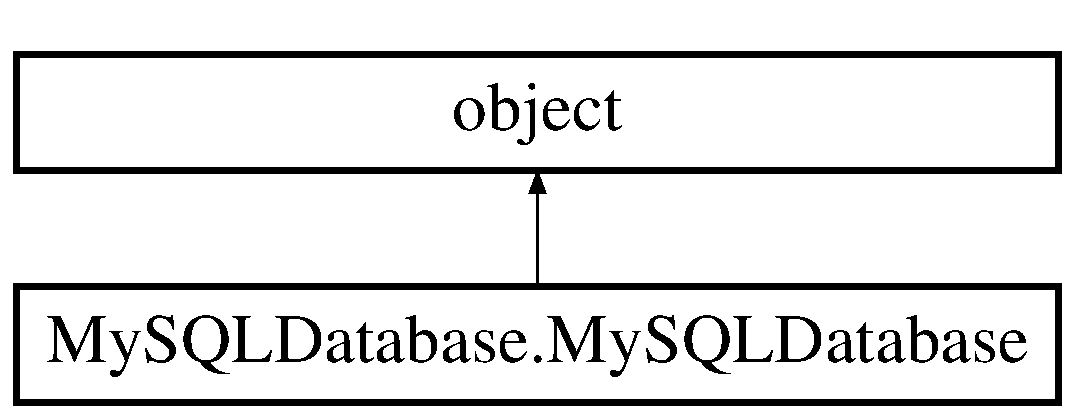
\includegraphics[height=2.000000cm]{class_my_s_q_l_database_1_1_my_s_q_l_database}
\end{center}
\end{figure}
\subsection*{Public Member Functions}
\begin{DoxyCompactItemize}
\item 
\hypertarget{class_my_s_q_l_database_1_1_my_s_q_l_database_ad83ed0d272a4c0c7949306cdcdfee5c3}{}\label{class_my_s_q_l_database_1_1_my_s_q_l_database_ad83ed0d272a4c0c7949306cdcdfee5c3} 
def {\bfseries \+\_\+\+\_\+init\+\_\+\+\_\+} (self, user\+Login\+Details)
\item 
def \hyperlink{class_my_s_q_l_database_1_1_my_s_q_l_database_ac9c6bc35283d4bfeacf4394937c625de}{login} (self)
\item 
\hypertarget{class_my_s_q_l_database_1_1_my_s_q_l_database_a1a94c4c47c41d928c10aa1e759d960b1}{}\label{class_my_s_q_l_database_1_1_my_s_q_l_database_a1a94c4c47c41d928c10aa1e759d960b1} 
def {\bfseries method\+Finder} (self)
\item 
def \hyperlink{class_my_s_q_l_database_1_1_my_s_q_l_database_a0fbc0754105eb3364e880b20c384a8dd}{main\+Logic} (self)
\item 
\hypertarget{class_my_s_q_l_database_1_1_my_s_q_l_database_ae5aafab03293ac07bd93a42cd7dbe2bf}{}\label{class_my_s_q_l_database_1_1_my_s_q_l_database_ae5aafab03293ac07bd93a42cd7dbe2bf} 
def {\bfseries exit\+Program} (self)
\item 
def \hyperlink{class_my_s_q_l_database_1_1_my_s_q_l_database_a3350d0f83d2d015b46bba5c0358a540d}{print\+Menu} (self)
\item 
def \hyperlink{class_my_s_q_l_database_1_1_my_s_q_l_database_a01cc9f1c3e782ada4c437682ae31c14c}{get\+Menu\+Input} (self)
\item 
def \hyperlink{class_my_s_q_l_database_1_1_my_s_q_l_database_ac7c560ff26c7d9295c4632385f61ce6d}{to\+C\+SV} (self, dates, ratings)
\item 
def \hyperlink{class_my_s_q_l_database_1_1_my_s_q_l_database_a746a62e1c7d7b11e7f00bbcbd92ed860}{custom\+Query} (self, G\+UI, query)
\end{DoxyCompactItemize}
\subsection*{Public Attributes}
\begin{DoxyCompactItemize}
\item 
\hypertarget{class_my_s_q_l_database_1_1_my_s_q_l_database_ae53f2dc61fcf32ccc89c5a65a3cf339e}{}\label{class_my_s_q_l_database_1_1_my_s_q_l_database_ae53f2dc61fcf32ccc89c5a65a3cf339e} 
{\bfseries menu\+Option}
\item 
\hypertarget{class_my_s_q_l_database_1_1_my_s_q_l_database_a5c64210f80c8a8fcfcc91dd0bf8150fa}{}\label{class_my_s_q_l_database_1_1_my_s_q_l_database_a5c64210f80c8a8fcfcc91dd0bf8150fa} 
{\bfseries username}
\item 
\hypertarget{class_my_s_q_l_database_1_1_my_s_q_l_database_a495a5f090202b50929b3efaa439e5c48}{}\label{class_my_s_q_l_database_1_1_my_s_q_l_database_a495a5f090202b50929b3efaa439e5c48} 
{\bfseries password}
\item 
\hypertarget{class_my_s_q_l_database_1_1_my_s_q_l_database_a786b536b34b946de38df9d9f21cee5a3}{}\label{class_my_s_q_l_database_1_1_my_s_q_l_database_a786b536b34b946de38df9d9f21cee5a3} 
{\bfseries back\+To\+Main}
\item 
\hypertarget{class_my_s_q_l_database_1_1_my_s_q_l_database_a8b542c607678f5e7b5374729ea8ec3a3}{}\label{class_my_s_q_l_database_1_1_my_s_q_l_database_a8b542c607678f5e7b5374729ea8ec3a3} 
{\bfseries db}
\item 
\hypertarget{class_my_s_q_l_database_1_1_my_s_q_l_database_ae41a0779e98d868bc7ec66f5f3f6fc74}{}\label{class_my_s_q_l_database_1_1_my_s_q_l_database_ae41a0779e98d868bc7ec66f5f3f6fc74} 
{\bfseries run\+\_\+query\+\_\+obj}
\item 
\hypertarget{class_my_s_q_l_database_1_1_my_s_q_l_database_ac712f257d654fe875e310818c7eb323f}{}\label{class_my_s_q_l_database_1_1_my_s_q_l_database_ac712f257d654fe875e310818c7eb323f} 
{\bfseries menu\+Lines}
\item 
\hypertarget{class_my_s_q_l_database_1_1_my_s_q_l_database_a6d93b8694aab750cb9138294e2046dec}{}\label{class_my_s_q_l_database_1_1_my_s_q_l_database_a6d93b8694aab750cb9138294e2046dec} 
{\bfseries logger}
\end{DoxyCompactItemize}


\subsection{Detailed Description}
\begin{DoxyVerb}Database: Holds the database object used for querying, also holds the
    logic for the menus and runs the actual queries. \end{DoxyVerb}
 

\subsection{Member Function Documentation}
\hypertarget{class_my_s_q_l_database_1_1_my_s_q_l_database_a746a62e1c7d7b11e7f00bbcbd92ed860}{}\label{class_my_s_q_l_database_1_1_my_s_q_l_database_a746a62e1c7d7b11e7f00bbcbd92ed860} 
\index{My\+S\+Q\+L\+Database\+::\+My\+S\+Q\+L\+Database@{My\+S\+Q\+L\+Database\+::\+My\+S\+Q\+L\+Database}!custom\+Query@{custom\+Query}}
\index{custom\+Query@{custom\+Query}!My\+S\+Q\+L\+Database\+::\+My\+S\+Q\+L\+Database@{My\+S\+Q\+L\+Database\+::\+My\+S\+Q\+L\+Database}}
\subsubsection{\texorpdfstring{custom\+Query()}{customQuery()}}
{\footnotesize\ttfamily def My\+S\+Q\+L\+Database.\+My\+S\+Q\+L\+Database.\+custom\+Query (\begin{DoxyParamCaption}\item[{}]{self,  }\item[{}]{G\+UI,  }\item[{}]{query }\end{DoxyParamCaption})}

\begin{DoxyVerb}customeQuery: Executes user custom query. Need validation here. \end{DoxyVerb}
 \hypertarget{class_my_s_q_l_database_1_1_my_s_q_l_database_a01cc9f1c3e782ada4c437682ae31c14c}{}\label{class_my_s_q_l_database_1_1_my_s_q_l_database_a01cc9f1c3e782ada4c437682ae31c14c} 
\index{My\+S\+Q\+L\+Database\+::\+My\+S\+Q\+L\+Database@{My\+S\+Q\+L\+Database\+::\+My\+S\+Q\+L\+Database}!get\+Menu\+Input@{get\+Menu\+Input}}
\index{get\+Menu\+Input@{get\+Menu\+Input}!My\+S\+Q\+L\+Database\+::\+My\+S\+Q\+L\+Database@{My\+S\+Q\+L\+Database\+::\+My\+S\+Q\+L\+Database}}
\subsubsection{\texorpdfstring{get\+Menu\+Input()}{getMenuInput()}}
{\footnotesize\ttfamily def My\+S\+Q\+L\+Database.\+My\+S\+Q\+L\+Database.\+get\+Menu\+Input (\begin{DoxyParamCaption}\item[{}]{self }\end{DoxyParamCaption})}

\begin{DoxyVerb}getMenuInput: Gets and validates user input of menu choice. \end{DoxyVerb}
 \hypertarget{class_my_s_q_l_database_1_1_my_s_q_l_database_ac9c6bc35283d4bfeacf4394937c625de}{}\label{class_my_s_q_l_database_1_1_my_s_q_l_database_ac9c6bc35283d4bfeacf4394937c625de} 
\index{My\+S\+Q\+L\+Database\+::\+My\+S\+Q\+L\+Database@{My\+S\+Q\+L\+Database\+::\+My\+S\+Q\+L\+Database}!login@{login}}
\index{login@{login}!My\+S\+Q\+L\+Database\+::\+My\+S\+Q\+L\+Database@{My\+S\+Q\+L\+Database\+::\+My\+S\+Q\+L\+Database}}
\subsubsection{\texorpdfstring{login()}{login()}}
{\footnotesize\ttfamily def My\+S\+Q\+L\+Database.\+My\+S\+Q\+L\+Database.\+login (\begin{DoxyParamCaption}\item[{}]{self }\end{DoxyParamCaption})}

\begin{DoxyVerb}login: Try/Except to log the user in. \end{DoxyVerb}
 \hypertarget{class_my_s_q_l_database_1_1_my_s_q_l_database_a0fbc0754105eb3364e880b20c384a8dd}{}\label{class_my_s_q_l_database_1_1_my_s_q_l_database_a0fbc0754105eb3364e880b20c384a8dd} 
\index{My\+S\+Q\+L\+Database\+::\+My\+S\+Q\+L\+Database@{My\+S\+Q\+L\+Database\+::\+My\+S\+Q\+L\+Database}!main\+Logic@{main\+Logic}}
\index{main\+Logic@{main\+Logic}!My\+S\+Q\+L\+Database\+::\+My\+S\+Q\+L\+Database@{My\+S\+Q\+L\+Database\+::\+My\+S\+Q\+L\+Database}}
\subsubsection{\texorpdfstring{main\+Logic()}{mainLogic()}}
{\footnotesize\ttfamily def My\+S\+Q\+L\+Database.\+My\+S\+Q\+L\+Database.\+main\+Logic (\begin{DoxyParamCaption}\item[{}]{self }\end{DoxyParamCaption})}

\begin{DoxyVerb}mainLogic: Holds the logic for the main menu. \end{DoxyVerb}
 \hypertarget{class_my_s_q_l_database_1_1_my_s_q_l_database_a3350d0f83d2d015b46bba5c0358a540d}{}\label{class_my_s_q_l_database_1_1_my_s_q_l_database_a3350d0f83d2d015b46bba5c0358a540d} 
\index{My\+S\+Q\+L\+Database\+::\+My\+S\+Q\+L\+Database@{My\+S\+Q\+L\+Database\+::\+My\+S\+Q\+L\+Database}!print\+Menu@{print\+Menu}}
\index{print\+Menu@{print\+Menu}!My\+S\+Q\+L\+Database\+::\+My\+S\+Q\+L\+Database@{My\+S\+Q\+L\+Database\+::\+My\+S\+Q\+L\+Database}}
\subsubsection{\texorpdfstring{print\+Menu()}{printMenu()}}
{\footnotesize\ttfamily def My\+S\+Q\+L\+Database.\+My\+S\+Q\+L\+Database.\+print\+Menu (\begin{DoxyParamCaption}\item[{}]{self }\end{DoxyParamCaption})}

\begin{DoxyVerb}printMenu: Prints the main menu. \end{DoxyVerb}
 \hypertarget{class_my_s_q_l_database_1_1_my_s_q_l_database_ac7c560ff26c7d9295c4632385f61ce6d}{}\label{class_my_s_q_l_database_1_1_my_s_q_l_database_ac7c560ff26c7d9295c4632385f61ce6d} 
\index{My\+S\+Q\+L\+Database\+::\+My\+S\+Q\+L\+Database@{My\+S\+Q\+L\+Database\+::\+My\+S\+Q\+L\+Database}!to\+C\+SV@{to\+C\+SV}}
\index{to\+C\+SV@{to\+C\+SV}!My\+S\+Q\+L\+Database\+::\+My\+S\+Q\+L\+Database@{My\+S\+Q\+L\+Database\+::\+My\+S\+Q\+L\+Database}}
\subsubsection{\texorpdfstring{to\+C\+S\+V()}{toCSV()}}
{\footnotesize\ttfamily def My\+S\+Q\+L\+Database.\+My\+S\+Q\+L\+Database.\+to\+C\+SV (\begin{DoxyParamCaption}\item[{}]{self,  }\item[{}]{dates,  }\item[{}]{ratings }\end{DoxyParamCaption})}

\begin{DoxyVerb}toCSV: Writes dates/ratings to CSV file.  \end{DoxyVerb}
 

The documentation for this class was generated from the following file\+:\begin{DoxyCompactItemize}
\item 
src/sql\+Database/My\+S\+Q\+L\+Database.\+py\end{DoxyCompactItemize}

\hypertarget{class_mongo_queries_1_1_online_reviews}{}\section{Mongo\+Queries.\+Online\+Reviews Class Reference}
\label{class_mongo_queries_1_1_online_reviews}\index{Mongo\+Queries.\+Online\+Reviews@{Mongo\+Queries.\+Online\+Reviews}}
\subsection*{Public Member Functions}
\begin{DoxyCompactItemize}
\item 
\hypertarget{class_mongo_queries_1_1_online_reviews_a6f3d0736bb3e7890a007e2d4823a6d0d}{}\label{class_mongo_queries_1_1_online_reviews_a6f3d0736bb3e7890a007e2d4823a6d0d} 
def \hyperlink{class_mongo_queries_1_1_online_reviews_a6f3d0736bb3e7890a007e2d4823a6d0d}{get\+Online\+Reviews} (i)
\begin{DoxyCompactList}\small\item\em accesses \hyperlink{class_mongo_queries_1_1_online_reviews}{Online\+Reviews} Collection \#\#\#\#\# \end{DoxyCompactList}\item 
\hypertarget{class_mongo_queries_1_1_online_reviews_a87dae9b1fdb0f48556e4835d102bb398}{}\label{class_mongo_queries_1_1_online_reviews_a87dae9b1fdb0f48556e4835d102bb398} 
def {\bfseries get\+Online\+Review\+Scores} (i)
\end{DoxyCompactItemize}


The documentation for this class was generated from the following file\+:\begin{DoxyCompactItemize}
\item 
src/mongo\+Database/Mongo\+Queries.\+py\end{DoxyCompactItemize}

\hypertarget{class_mongo_queries_1_1_product_details}{}\section{Mongo\+Queries.\+Product\+Details Class Reference}
\label{class_mongo_queries_1_1_product_details}\index{Mongo\+Queries.\+Product\+Details@{Mongo\+Queries.\+Product\+Details}}
\subsection*{Public Member Functions}
\begin{DoxyCompactItemize}
\item 
\hypertarget{class_mongo_queries_1_1_product_details_acfcdac1a1f030b4753d91ff1e763dab2}{}\label{class_mongo_queries_1_1_product_details_acfcdac1a1f030b4753d91ff1e763dab2} 
def \hyperlink{class_mongo_queries_1_1_product_details_acfcdac1a1f030b4753d91ff1e763dab2}{get\+Product\+Details} (i)
\begin{DoxyCompactList}\small\item\em accesses \hyperlink{class_mongo_queries_1_1_product_details}{Product\+Details} Collection \#\#\#\#\# \end{DoxyCompactList}\item 
\hypertarget{class_mongo_queries_1_1_product_details_a3eb00d0b74e93e53d2760879a3bf2032}{}\label{class_mongo_queries_1_1_product_details_a3eb00d0b74e93e53d2760879a3bf2032} 
def {\bfseries get\+Product\+Name} (i)
\item 
\hypertarget{class_mongo_queries_1_1_product_details_a5c2c0e637a07d05736758bc59b85312e}{}\label{class_mongo_queries_1_1_product_details_a5c2c0e637a07d05736758bc59b85312e} 
def {\bfseries get\+Product\+Description} (i)
\end{DoxyCompactItemize}


The documentation for this class was generated from the following file\+:\begin{DoxyCompactItemize}
\item 
src/mongo\+Database/Mongo\+Queries.\+py\end{DoxyCompactItemize}

\hypertarget{class_mongo_queries_1_1_user_stories}{}\section{Mongo\+Queries.\+User\+Stories Class Reference}
\label{class_mongo_queries_1_1_user_stories}\index{Mongo\+Queries.\+User\+Stories@{Mongo\+Queries.\+User\+Stories}}
\subsection*{Public Member Functions}
\begin{DoxyCompactItemize}
\item 
\hypertarget{class_mongo_queries_1_1_user_stories_a96555ca89afb9902322c4fc75d56ed23}{}\label{class_mongo_queries_1_1_user_stories_a96555ca89afb9902322c4fc75d56ed23} 
def {\bfseries average\+Rating\+For\+Customer} (i)
\item 
\hypertarget{class_mongo_queries_1_1_user_stories_a92619d4a0c2ffabe1b6d1df13f5bd778}{}\label{class_mongo_queries_1_1_user_stories_a92619d4a0c2ffabe1b6d1df13f5bd778} 
def {\bfseries average\+Rating\+For\+Product} (i)
\item 
\hypertarget{class_mongo_queries_1_1_user_stories_a2d8360b85d038a7f6939810758619a17}{}\label{class_mongo_queries_1_1_user_stories_a2d8360b85d038a7f6939810758619a17} 
def {\bfseries delivery\+Scores\+Over\+Time} ()
\item 
\hypertarget{class_mongo_queries_1_1_user_stories_a356dd82d446efd8db255a979310b256d}{}\label{class_mongo_queries_1_1_user_stories_a356dd82d446efd8db255a979310b256d} 
def {\bfseries customer\+Service\+Scores\+Over\+Time} ()
\end{DoxyCompactItemize}


The documentation for this class was generated from the following file\+:\begin{DoxyCompactItemize}
\item 
src/mongo\+Database/Mongo\+Queries.\+py\end{DoxyCompactItemize}

%--- End generated contents ---

% Index
\backmatter
\newpage
\phantomsection
\clearemptydoublepage
\addcontentsline{toc}{chapter}{Index}
\printindex

\end{document}
